% !TeX encoding = UTF-8
% !TeX spellcheck = en_US
\documentclass[twocolumn]{article}
\usepackage[cm]{fullpage}
\usepackage{yfonts}
\usepackage{moodlev5}
\usepackage{tikz}
\usepackage{varwidth}
\usepackage{hyperref}

\def\myequation{y=a\sqrt{x}+b}

\tikzstyle{pict} = [minimum height=1em,inner sep=0pt,execute at begin 
node={\begin{varwidth}{\linewidth}},
execute at end node={\end{varwidth}}]

\newcommand\embedaspict[1]{\begin{tikzpicture}\node[pict]{#1};\end{tikzpicture}}

\htmlregister{\myequation}
\htmlregister{\embedaspict}

\begin{document}

\section*{Introduction}

This document presents examples of questions that one can make with the 
\texttt{moodle} \LaTeX{} package as of version \texttt{0.5}, currently 
available on \href{https://ctan.org/pkg/moodle}{CTAN}.

\begin{quiz}[ % options that apply to all questions
%	points=1, % default 1
%	penalty=0, % penalty in case of wrong attempt (between 0 and 1). Default 0.1
%	fraction=0, % fraction of points for wrong or partially true answers
	%feedback={coucou}
	] {Example Quiz}

\begin{multi}[points=3,numbering=Alph]{Multiple Choice (single correct answer)}
% Numbering possibilities:
% - numbering=alph, alpha, or abc,
% - numbering=Alph, Alpha, or ABC, (broken at XML import)
% - numbering=arabic or 123,
% - numbering=roman or iii,
% - numbering=Roman or IIII,
% - numbering=none.
What is the first derivative of $x^3$ w.r.t. $x$?
\item[feedback={this is a very long feedback; it may even be displayed in
several lines. Here is a new sentence! Does that work? Yes.}] $\frac{1}{4} x^4+C$
\item[]* $3x^2$ % the star stands for fraction=1
\item[feedback={text}] $51$
\end{multi}

\begin{multi}[multiple,numbering=roman]{Multiple Choice (several correct 
answers)}
Select the following numbers that are prime.
\item[feedback={it is only divided by 1 and itself!}]* $\sqrt{25}$
\item[feedback={divided by 2 and 3!}] 6
\item[]* 7 %feedback={it is only divided by 1 and itself!}
\item[feedback={divided by 2 and 4! Normally this feedback would be short but I
want to make it longer for testing purposes.}] \embedaspict{8}
\end{multi}

\begin{numerical}[ % options that apply to all answers
%	points=1, % default 1
%	penalty=0, % penalty in case of wrong attempt (between 0 and 1). Default 0.1
%%	fraction=0, % fraction of points for wrong or partially true answers
tolerance=0.01
%	feedback={coucou} % feedback is given regardless of the answer
] {Numerical}
What is $8+3$?
\item[fraction=100,feedback={this is a very long feedback; it may even be 
displayed in several lines. Here is a new sentence! Does that work? Yes.}] 11
\item[fraction=0] 12
\item[fraction=0,feedback={Pfff}] 5
\end{numerical}

\begin{shortanswer}[case sensitive=true]{Short Answer (case sensitive)}
What was Newton's first name?
\item[feedback={this is a very long feedback; it may even be displayed in 
several lines. Here is a new sentence! Does that work? Yes.}] Isaac
\item[fraction=50,feedback={forgot how to capitalize properly?}] isaac
\item[fraction=0,feedback={how noble!}] Sir* % any answer 
%starting with "Sir"
\item[fraction=0,feedback={no...}] * % the asterisk represents any other answer
\end{shortanswer}

\begin{shortanswer}{Short Answer (case insensitive)}
Newton's rival was \embedaspict{\frakfamily Gottfried Wilhelm} \blank.
\item[feedback={Correct! But why the hell did you put a dot?}] Leibniz.
\item Leibniz
\item[fraction=0,feedback={write it backwards!}] Zinbiel
\item[fraction=0,feedback={ask wikipedia}] * % the asterisk represents any 
%other answer
\end{shortanswer}

\begin{matching}{Matching (standard)}
Answer-specific feedback is too complicated for matching questions (lots of 
possible combinations). Moodle does not support that\dots

In Moodle, the matching is made by selecting answers in a dropdown list. The 
latter only allows text: pictures cannot be placed and neither HTML nor LaTeX 
are rendered. 
	\item[feedback={this feedback is garbage: it is placed in the XML but won't 
	make it through the Moodle import}] Orange \answer Orange
	\item[feedback={Actually, Moodle's matching question type does not seem to 
	support feedback}] Lemon $\myequation$ \answer Yellow
	\item[feedback={sadly...}] Banana \answer Yellow
% "Yellow" is repeated twice but will appear only once in the offered answers
	\item[] Strawberry \answer Red
	\item[]  \answer Black
\end{matching}

\begin{matching}[dd]{Matching (drag and drop)}
This question type comes with a specific Moodle plugin. In the offered
answers, it allows to get LaTeX equations rendered. There is a bug that prevents 
pictures to be used in answers.
\item[feedback={this feedback is garbage: it is placed in the XML but won't 
make it through the Moodle import}] \embedaspict{Orange} \answer Orange
\item[feedback={Actually, Moodle's matching question type does not support
feedback}] Lemon $\myequation$ \answer Yellow
\item[feedback={sadly...}] Banana \answer Yellow
% "Yellow" is repeated twice but will appear only once in the offered answers
\item[] Strawberry \answer Red
\item[]  \answer Black $\myequation$
\end{matching}

\begin{essay}[response required,response format=text,template={put 
your answer here}]{Essay}
\embedaspict{Is learning worth it?}
\item if the answer is "yes" $\rightarrow$ full grade
\item if the answer is silly \embedaspict{$\rightarrow$} minimum grade
\end{essay}

\begin{cloze}{Cloze}
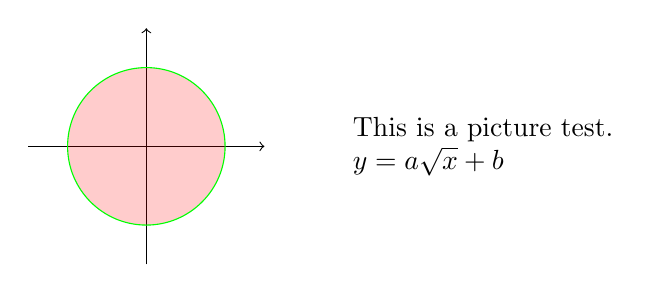
\begin{tikzpicture}
\draw[->] (-1.5,0)--(1.5,0);
\draw[->] (0,-1.5)--(0,1.5);
\draw[fill=red,fill opacity=.2,draw=green] (0,0)circle[radius=1];
\node[text width=3.5cm,anchor=west] at (2.5,0) {This is a picture test. 
$\myequation$};
\end{tikzpicture}
Within the cloze environment, when using multichoice, Moodle allows to make 
only one choice. Therefore, multiple choice questions shall be made such that 
all points can be acquired with a single good answer only. A limitation of 
Moodle's parser, discussed 
\href{https://moodle.org/mod/forum/discuss.php?d=275299}{here}, has to be 
overcome for math display in answers or feedbacks that contain closing curly 
braces ($\}$). It should be escaped with a $\backslash$.

\begin{multi}
First, an inline dropdown list. It is very compact on Moodle. The drawback is 
that there is no LaTeX or HTML rendering in answers. The feedback renders HMTL 
and LaTeX. It is a bit hidden as it pops up only when hovering the 
checkmark or X mark with the mouse.
\item[feedback={yes}]* chip
\item[fraction=10] chop
\item[feedback={this is a quite long feedback.}] chap
\end{multi}

\begin{multi}[horizontal]
Second, an horizontal multichoice. May be quite compact as well but inadequate 
when possible answers are lengthy or numerous. Both answers and feedback can 
be rendered using LaTeX and HTML.
\item[feedback={text}]* True
\item[] False
\item[feedback={silly!}] $y=ax+b$
\end{multi}

\begin{multi}[vertical]
Last, a vertical multichoice. Behaves like the standard single multichoice.
\item[feedback={yes!}]* yop
\item[fraction=20] yap
\item[feedback={no!}] yip
\item[feedback={nope...}] $yup$
\end{multi}
\end{cloze}

\end{quiz}

%\begin{quiz}{Second Quiz}	
%\begin{numerical}{Numerical}
%What is $1+1$?
%\item 2
%\end{numerical}	
%\end{quiz}

\end{document}
